Das Template des Signals kommt aus der Monte Carlo Simulation.
Dabei wird ausgenutzt, dass in der Simulation bekannt ist, wo welches Teilchen herkommt und welches Teilchen auf das EMCal trifft.
Dadurch wird ermöglicht genau bestimmen zu können, woher ein Photonkandidat stammt und ob es sich dabei um ein Photon oder ein konvertiertes Photon handelt.
\begin{figure}[tp]
\centering
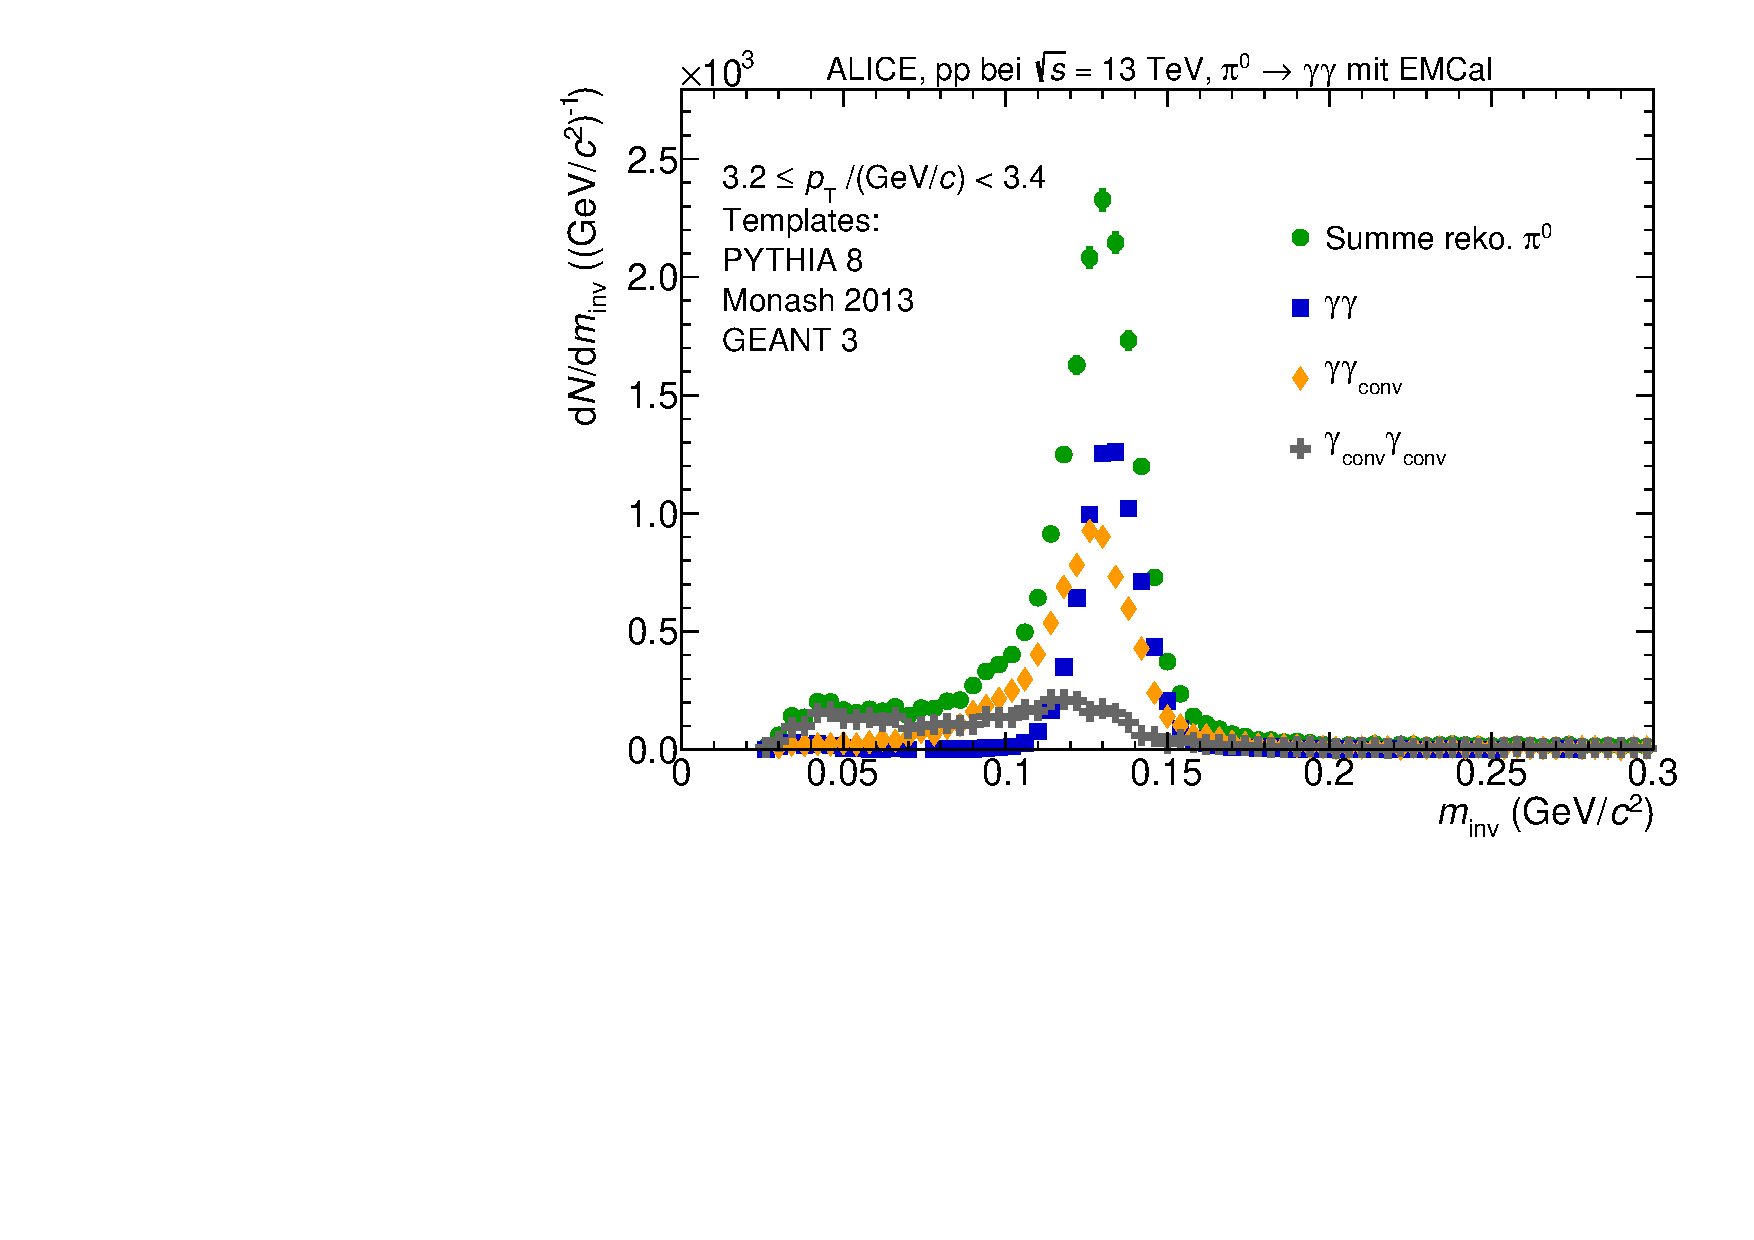
\includegraphics[width=.75\linewidth]{PeakTemplateMotivation10_Data_2016.pdf}
\caption{Template des Signals (grün) mit seinen drei Teilkomponenten.
Diese bestehen aus Kombinationen mit zwei Photonen (blau), einem Photon und einem konversions Elektron oder Positron (gelb) und zwei unterschiedlichen koversions Elektron oder Positron.}
\label{fig:SigTemp}
\end{figure}
\newline
Abbildung \ref{fig:SigTemp} zeigt das Template des Signals in grün, sowie die Aufteilung des Signals in einzelnen Komponenten.
Die Komponenten setzen sich aus den drei möglichen Kombinationen von Photonenkandidaten zusammen.
Zum einen aus Photonenkandidaten aus Photonen, in der Abbildung als $\gamma$ bezeichnet und zum anderen aus Photonenkandidaten aus einem Elektron oder Positron, die durch das konvertierten  eines Photonen entstanden.
Letztere werden in der Abbildung durch $\gamma_\text{conv}$ symbolisiert.
\newline
In blau sind die Kombinationen aus zwei Photonen ($\gamma\gamma$) dargestellt, in gelb die Kombination aus Photon und Elektron oder Positron ($\gamma\gamma_\text{conv}$) und in grau die Kombination aus koversions Elektron oder Positron miteinander ($\gamma_\text{conv}\gamma_\text{conv}$).
\newline
Die Abbildung zeigt außerdem, wie zuvor angesprochen, dass auch bei einer invarianten Masse um $0\,05 \text{ GeV}/c^{2}$ Signal vorliegt.
Der Anteil des Signals um diese invariante Masse besteht dominant aus zwei konvertierten Photonen.
Genau dieser Teil des Signals wird nicht durch die Standardmethode berücksichtigt.
Durch das Berücksichtigen in der Analyse mit Hilfe der Templates wird einer geringere statistische Unsicherheit erwartet.